\documentclass[12pt, a4paper]{article}

\usepackage[hmargin=2.5cm, vmargin=2cm]{geometry}
\usepackage{amsthm, amssymb, mathtools, yhmath, graphicx}
\usepackage{fontspec, type1cm, titlesec, titling, fancyhdr, tabularx}
\usepackage{color}
\usepackage{unicode-math}
\usepackage{float}
\usepackage{hhline}
\usepackage{comment}
\usepackage{siunitx}
\usepackage{csvsimple}
\usepackage{subcaption}

\usepackage[CheckSingle, CJKmath]{xeCJK}
\usepackage{CJKulem}
\usepackage{enumitem}
\usepackage{tikz}
\usepackage[siunitx]{circuitikz}
\usepackage{wrapfig}
%\setCJKmainfont[BoldFont=cwTex Q Hei]{cwTex Q Ming}
%\setCJKsansfont[BoldFont=cwTex Q Hei]{cwTex Q Ming}
%\setCJKmonofont[BoldFont=cwTex Q Hei]{cwTex Q Ming}
\setCJKmainfont[BoldFont=cwTeX Q Hei]{cwTeX Q Ming}

\def\normalsize{\fontsize{12}{18}\selectfont}
\def\large{\fontsize{14}{21}\selectfont}
\def\Large{\fontsize{16}{24}\selectfont}
\def\LARGE{\fontsize{18}{27}\selectfont}
\def\huge{\fontsize{20}{30}\selectfont}

%\titleformat{\section}{\bf\Large}{\arabic{section}}{24pt}{}
%\titleformat{\subsection}{\large}{\arabic{subsection}.}{12pt}{}
%\titlespacing*{\subsection}{0pt}{0pt}{1.5ex}

\parindent=24pt

\DeclarePairedDelimiter{\abs}{\lvert}{\rvert}
\DeclarePairedDelimiter{\norm}{\lVert}{\rVert}
\DeclarePairedDelimiter{\inpd}{\langle}{\rangle}
\DeclarePairedDelimiter{\ceil}{\lceil}{\rceil}
\DeclarePairedDelimiter{\floor}{\lfloor}{\rfloor}

\newcommand{\unit}[1]{\:(\text{#1})}
\newcommand{\df}[1]{\mathop{}\!\mathrm{d^#1}}
\newcommand{\img}{\mathrm{i}}

\title{ \bf {\Huge 電子電路實驗6:RCL 電路之步級響應}\\ 實驗結報}
\author{B02901178 江誠敏}
\date{2014/10/07} 

\begin{document}

\maketitle

\section{實驗結果}
\subsection{過阻尼}
\begin{figure}[H]
  \centering
  \begin{subfigure}[b]{0.4\textwidth}
    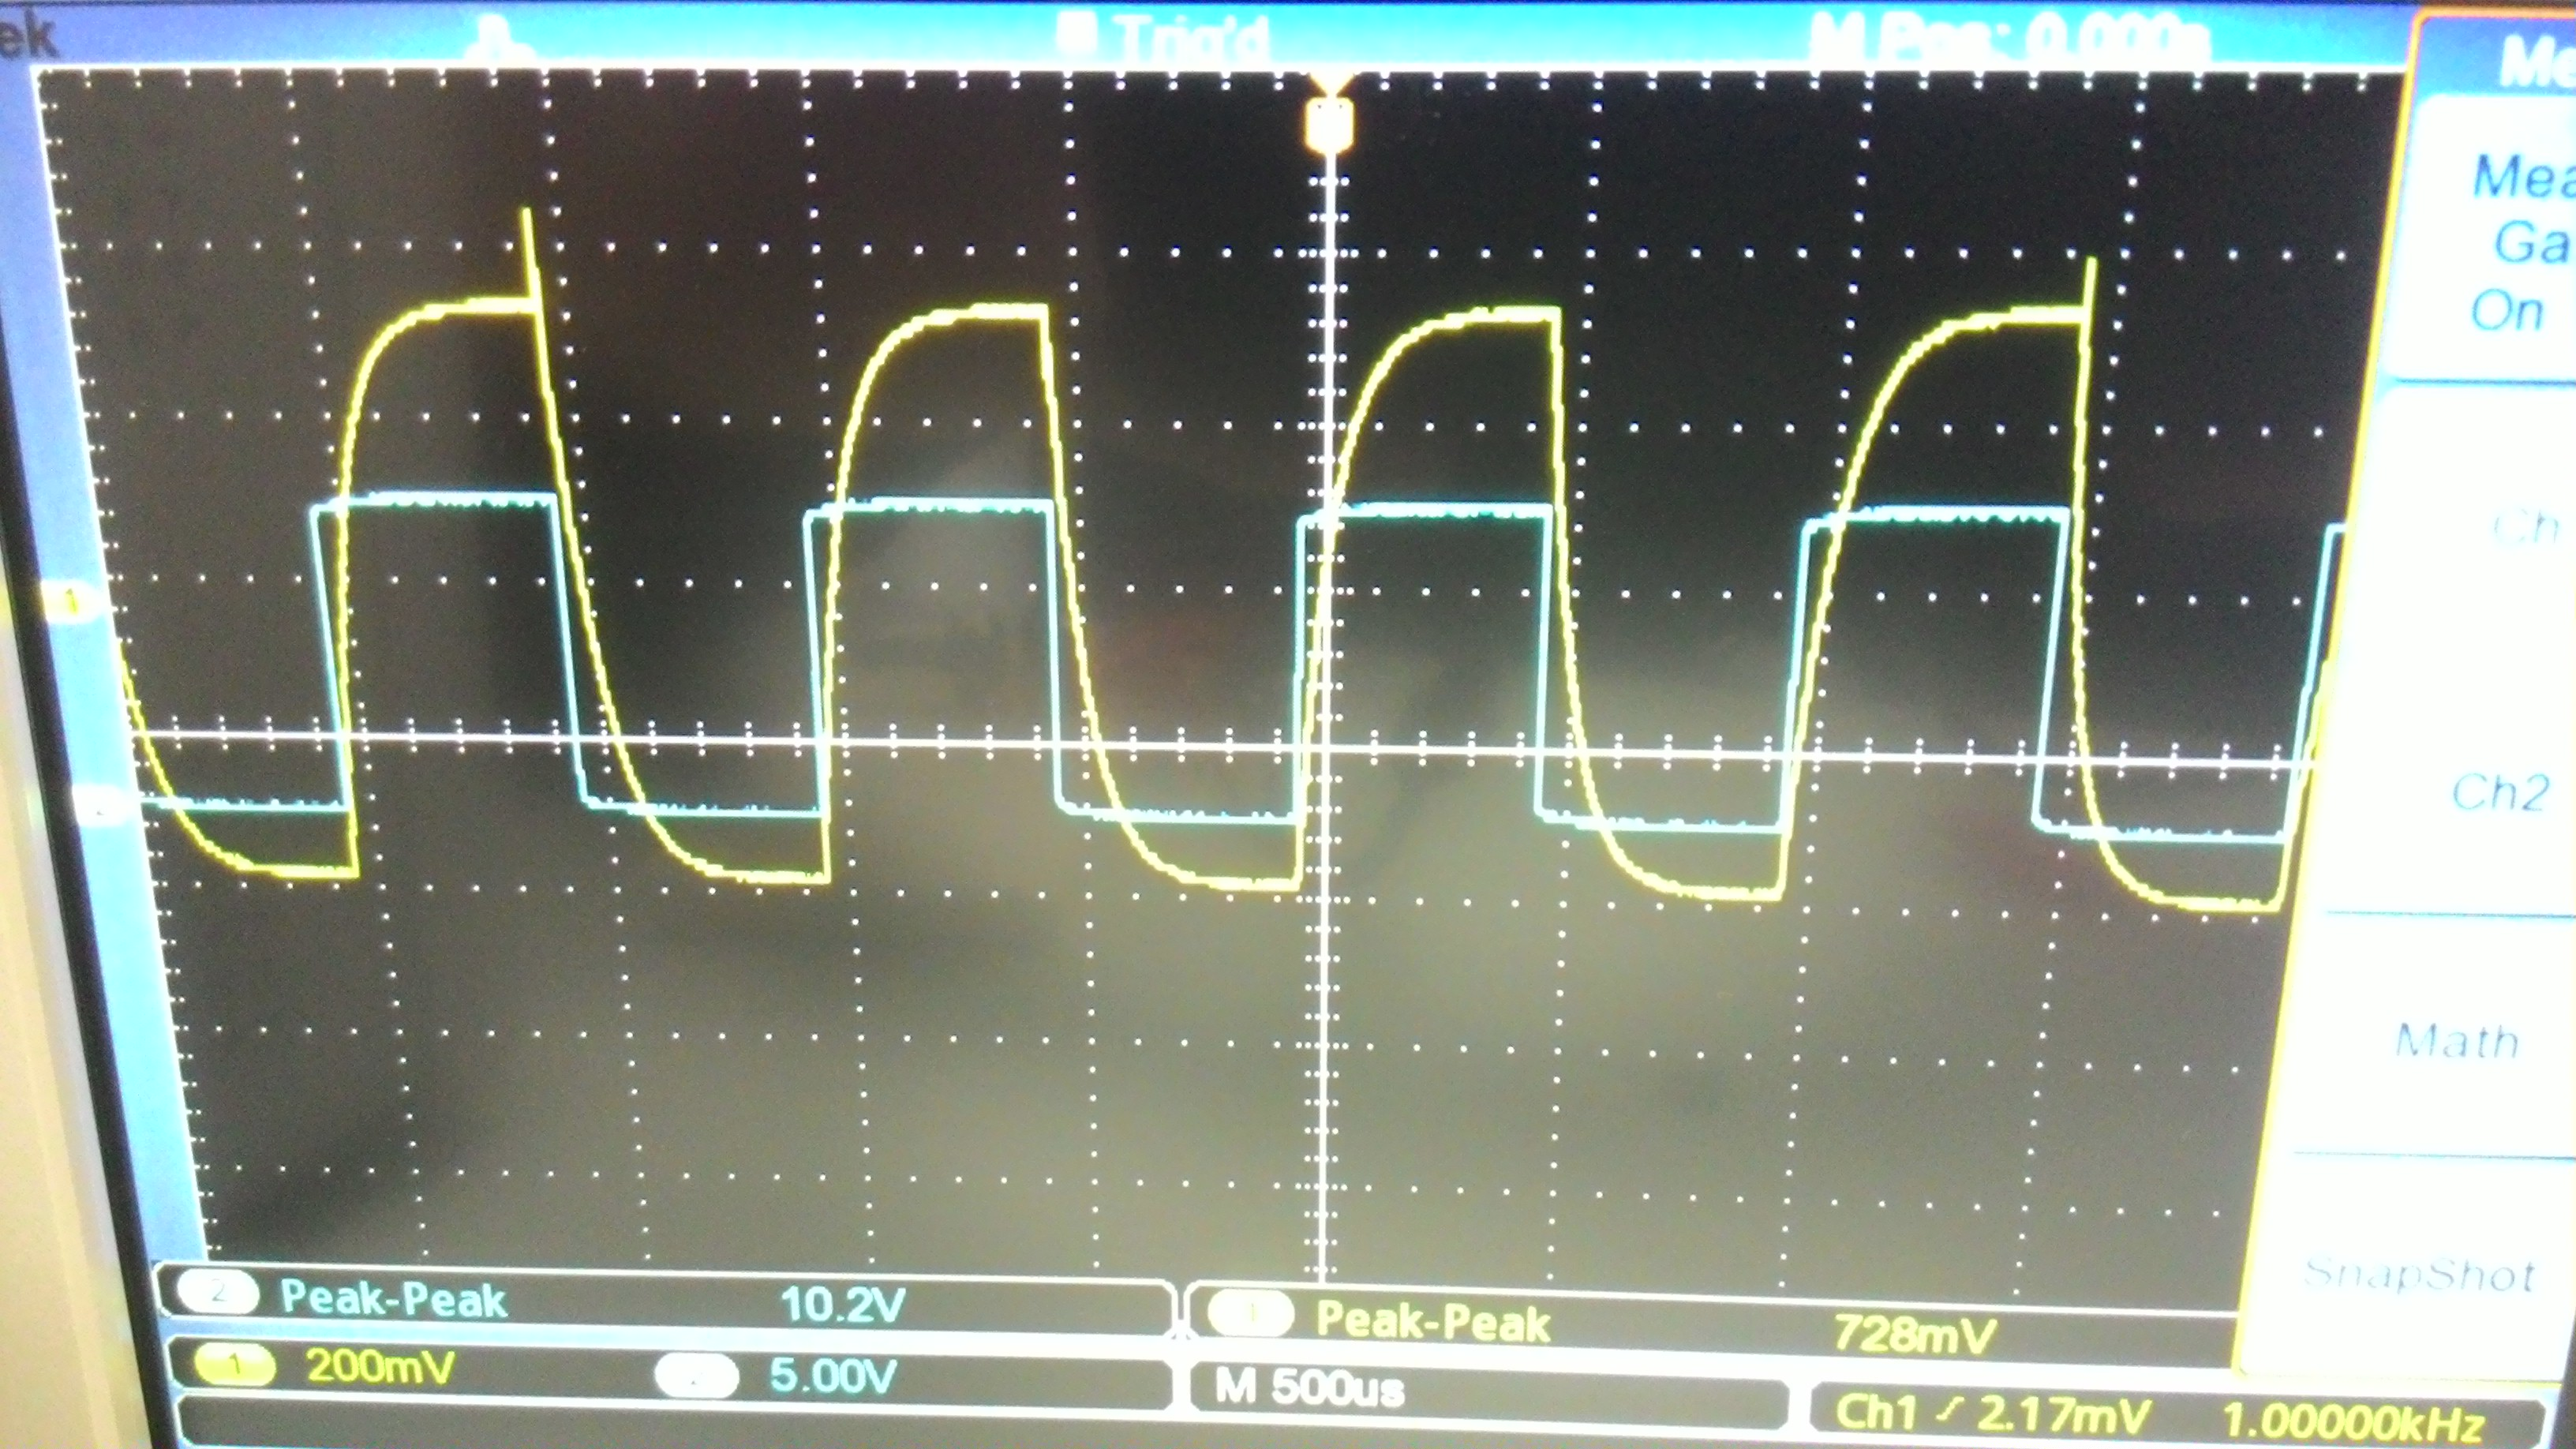
\includegraphics[width=1\textwidth]{data/pic/P_20141118_184858.jpg}
    \caption{$V_C$}
  \end{subfigure}
  ~
  \begin{subfigure}[b]{0.4\textwidth}
    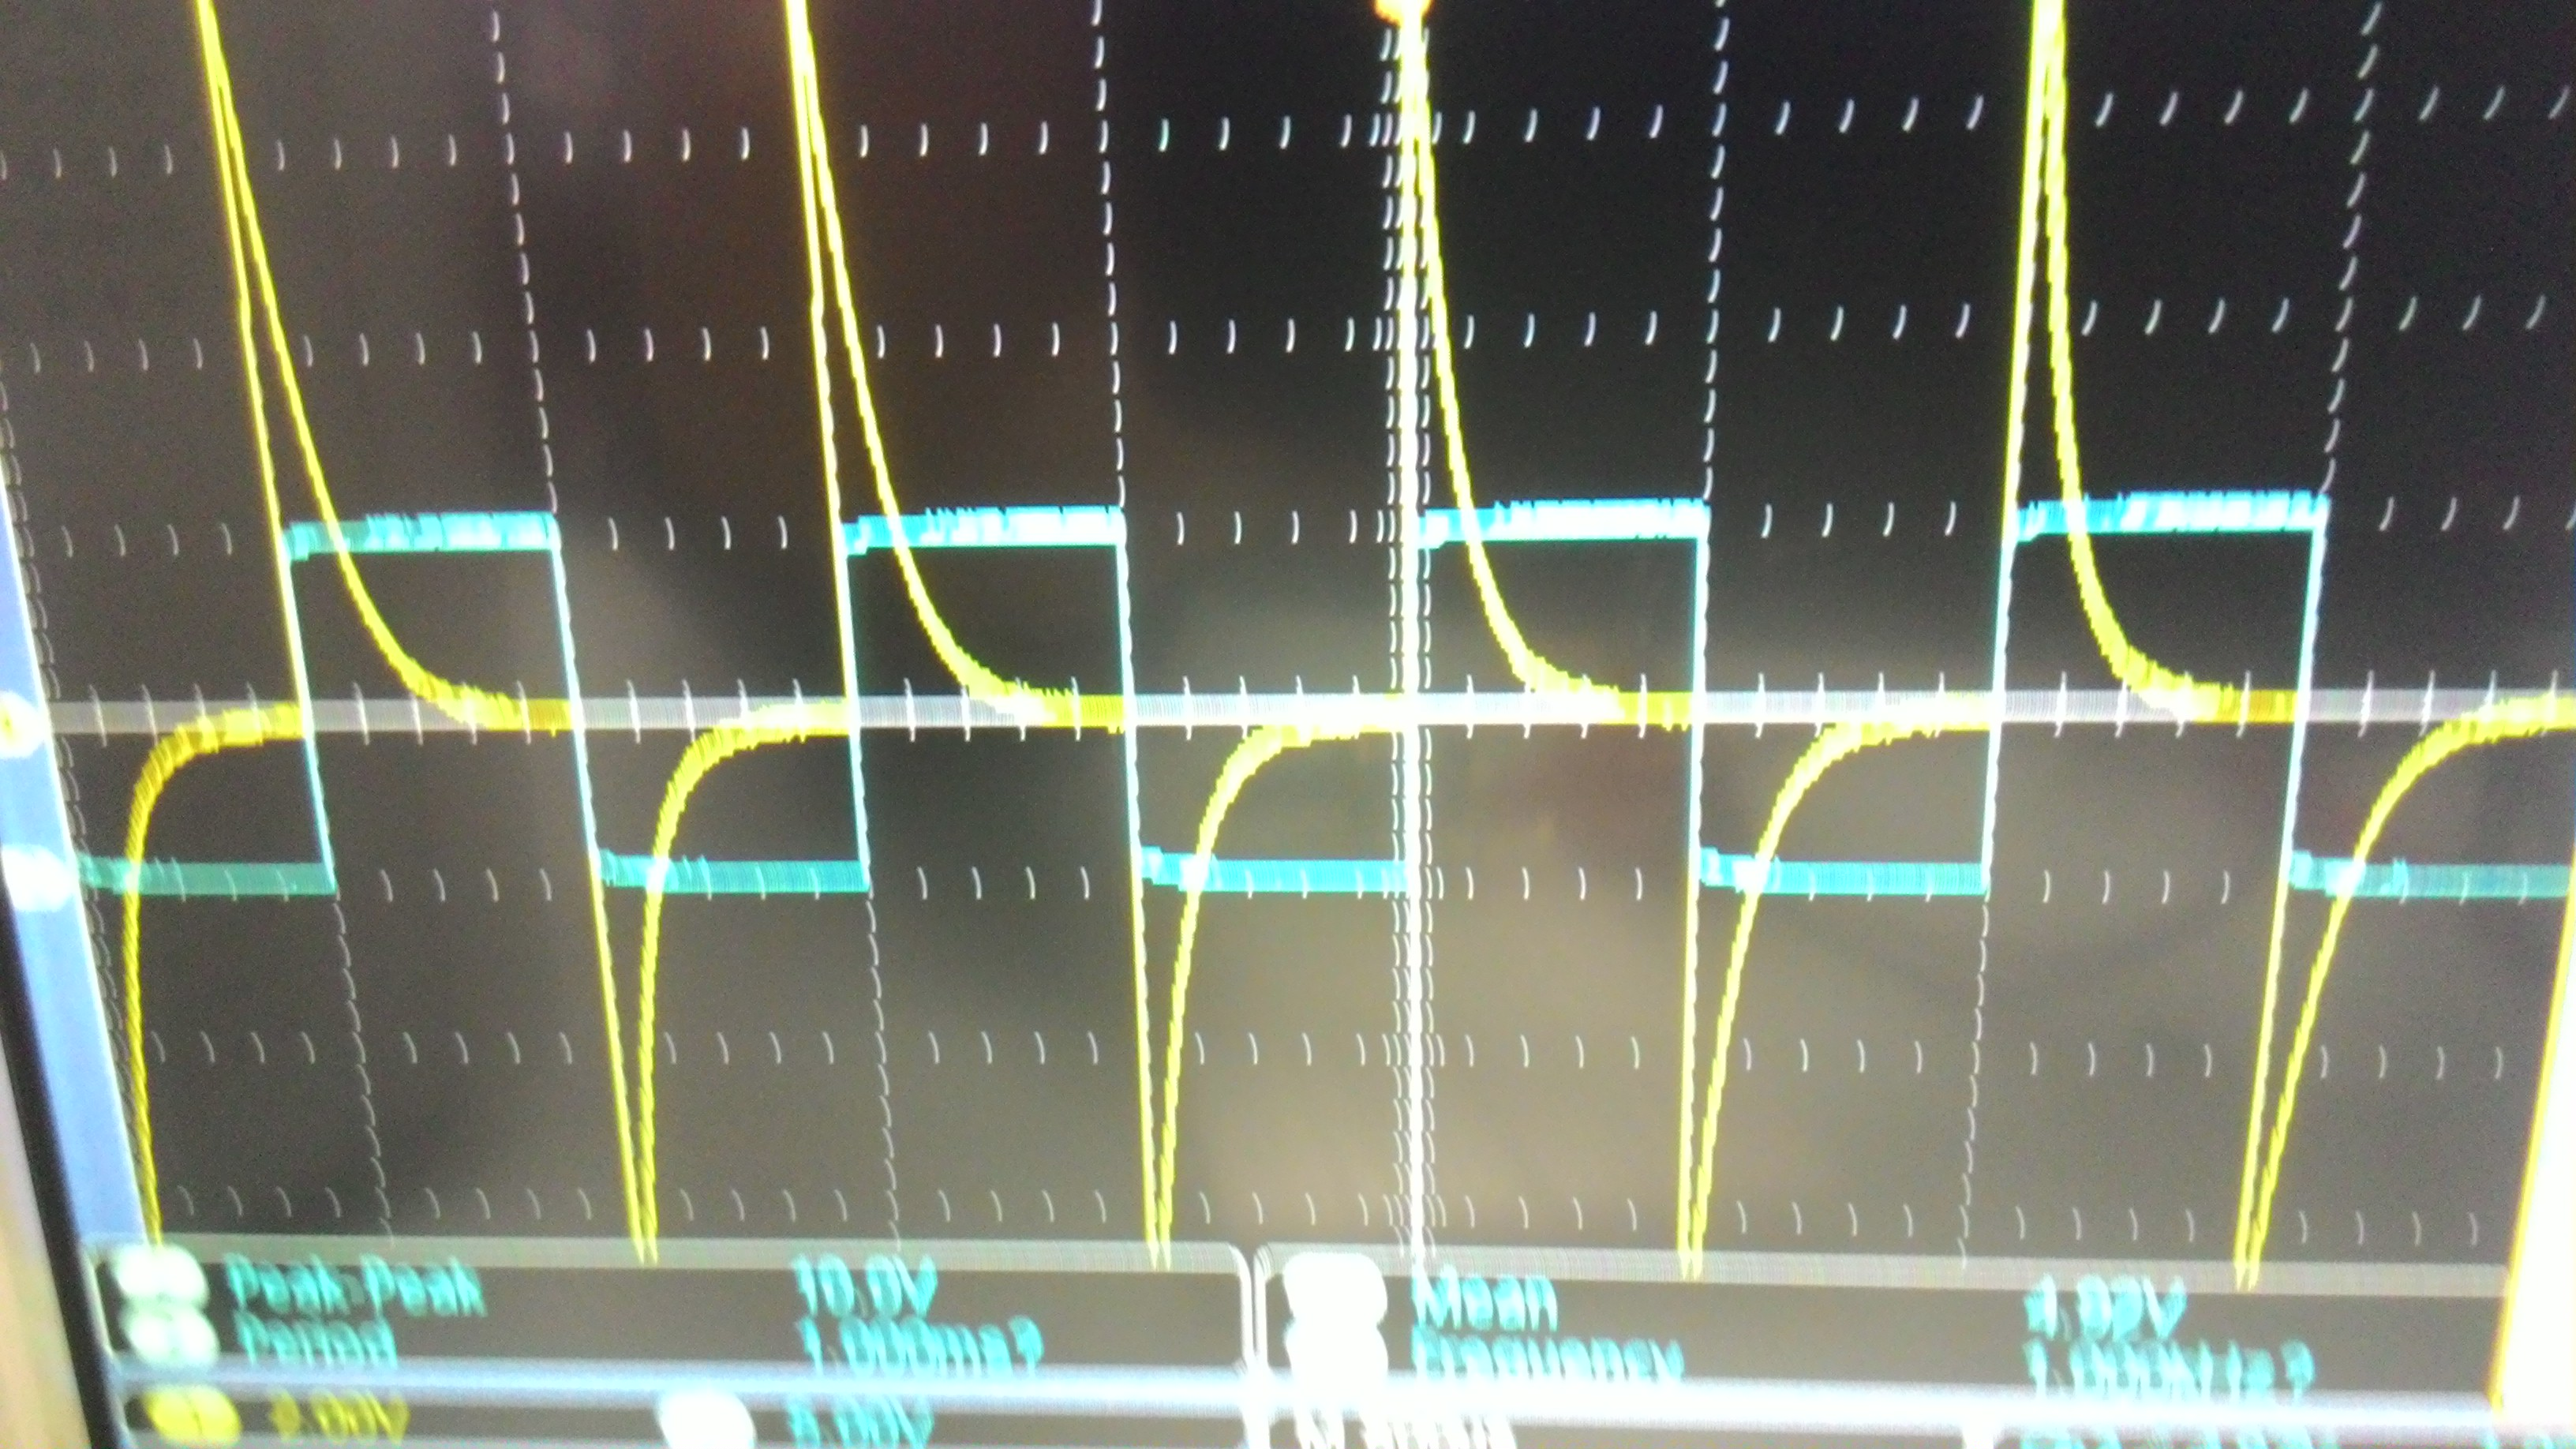
\includegraphics[width=1\textwidth]{data/pic/P_20141118_185319.jpg}
    \caption{$V_R$}
  \end{subfigure}
\end{figure}
$V_L$的照片不知為啥不見了…

\subsection{輕阻尼}
\begin{figure}[H]
  \centering
  \begin{subfigure}[b]{0.6\textwidth}
    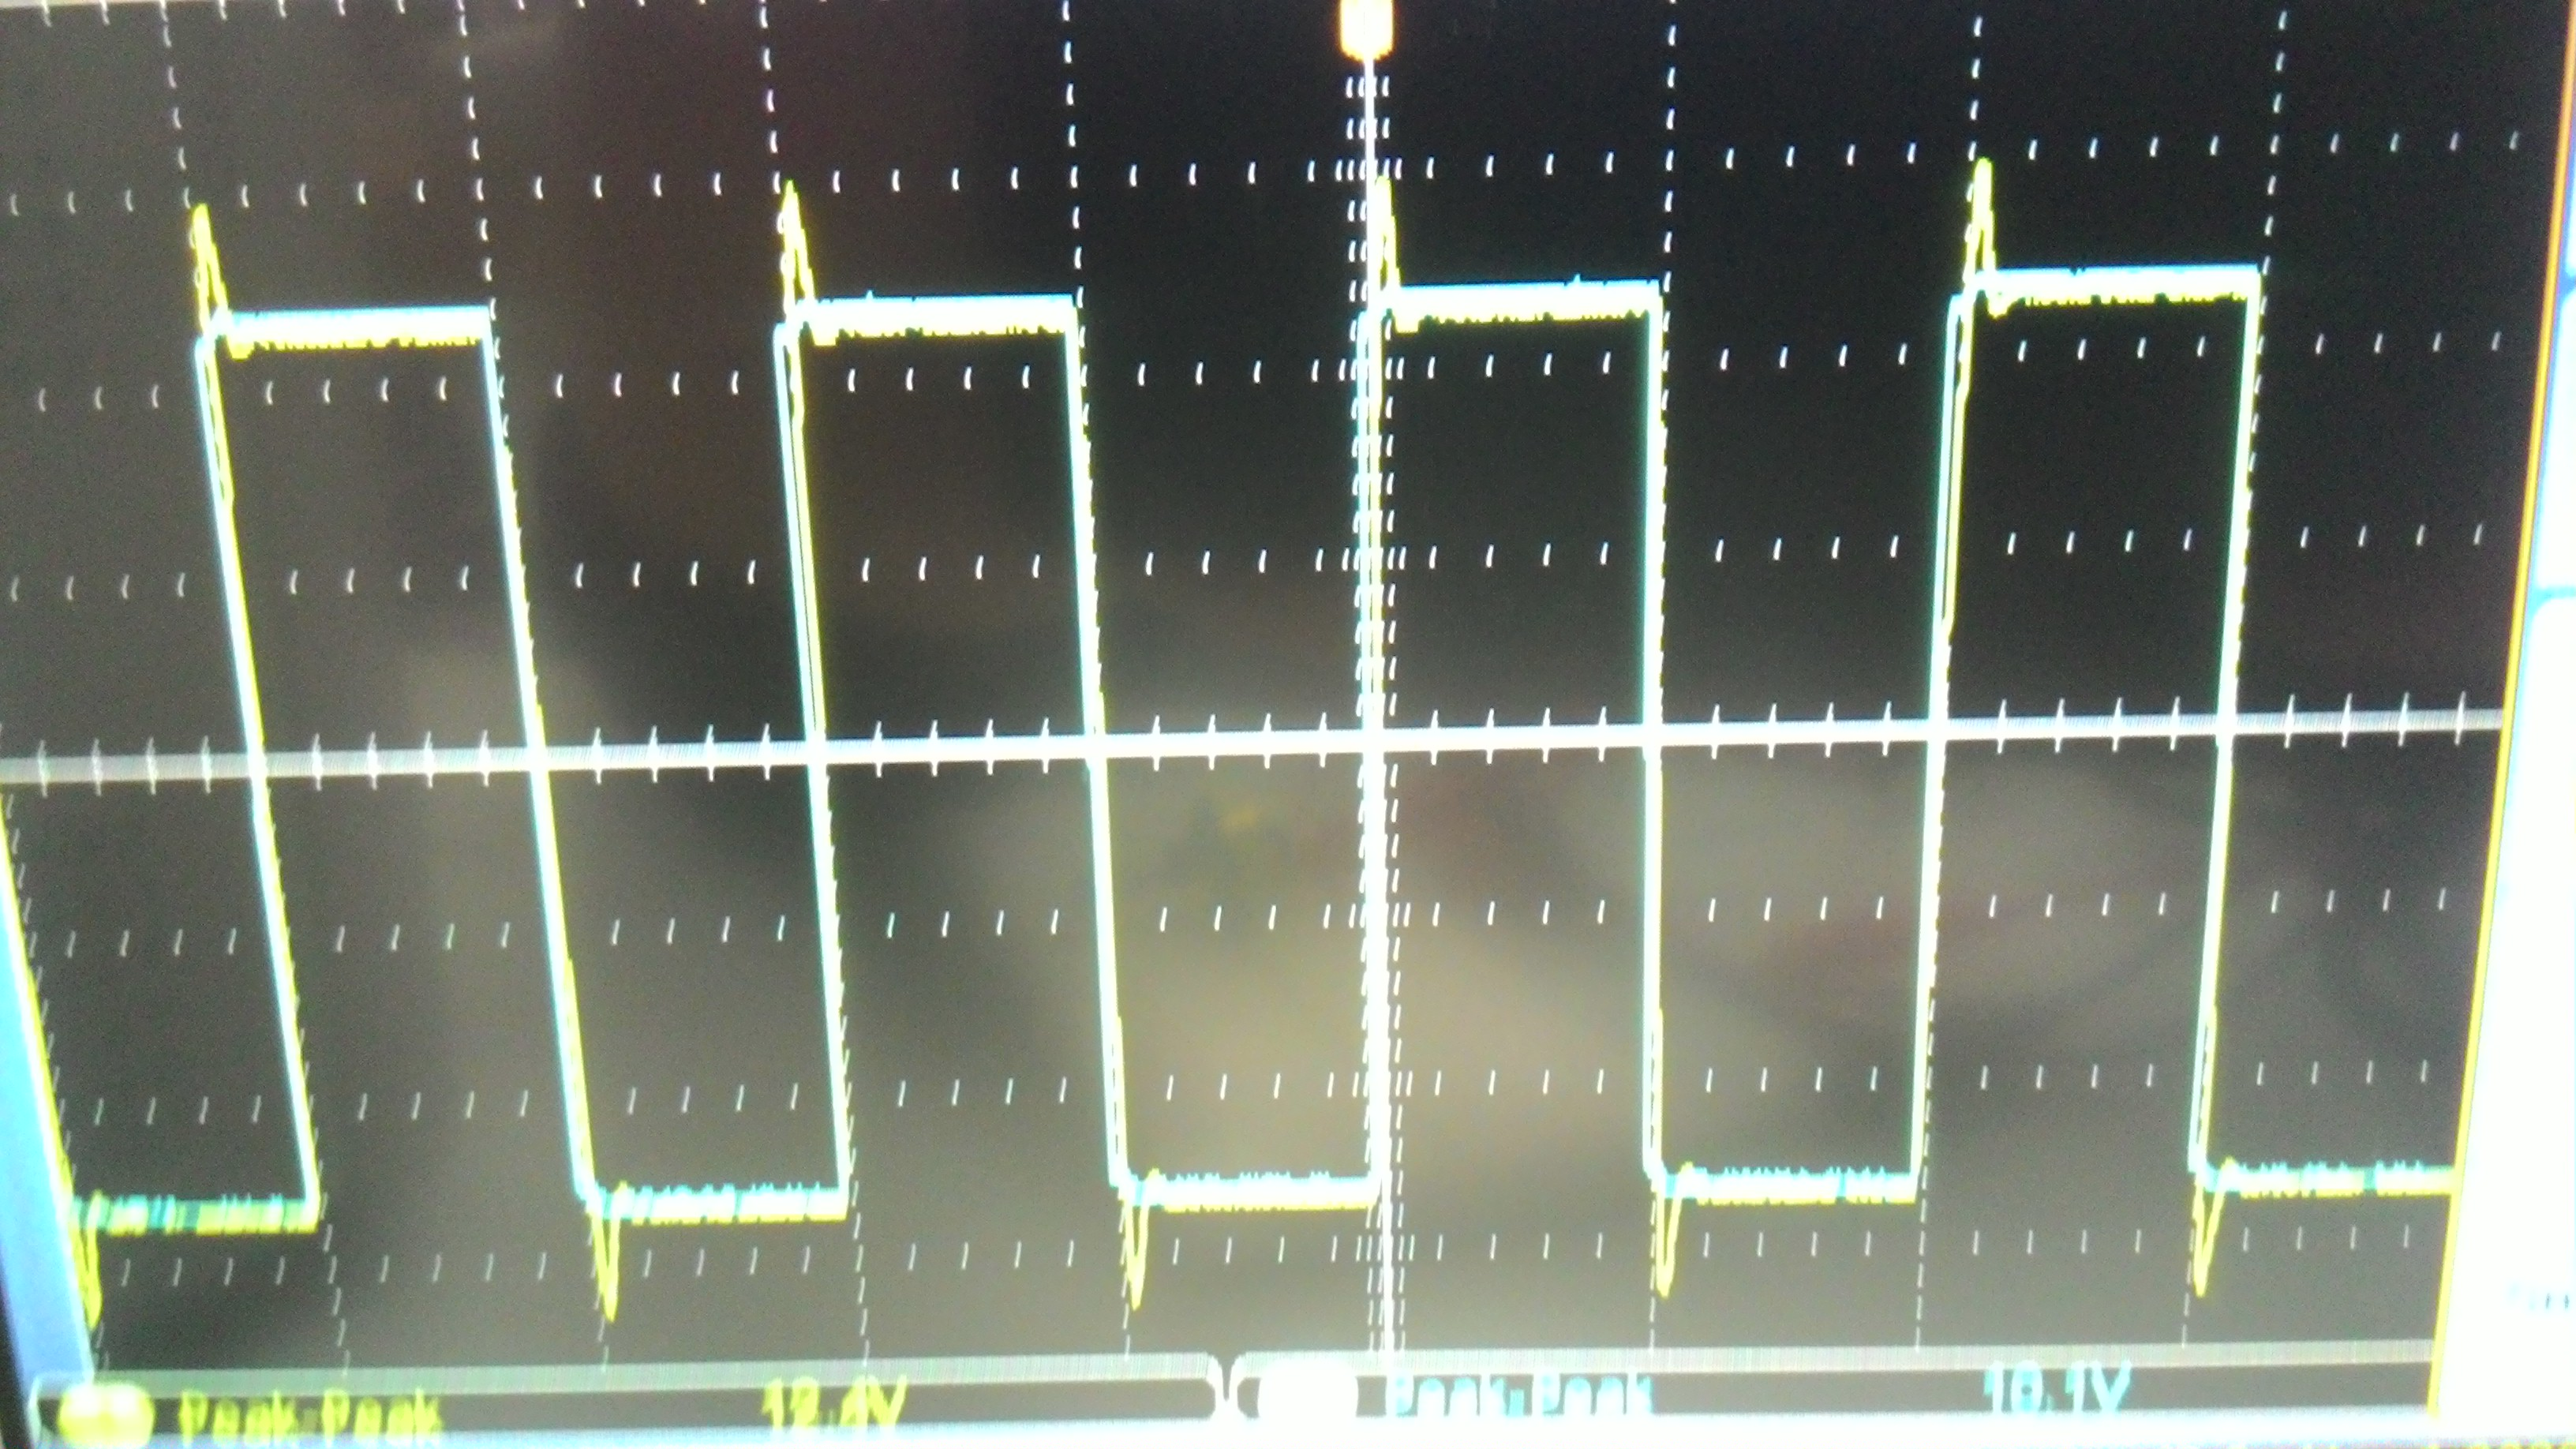
\includegraphics[width=1\textwidth]{data/pic/P_20141118_190608.jpg}
    \caption{$V_C$}
  \end{subfigure}
  \begin{subfigure}[b]{0.6\textwidth}
    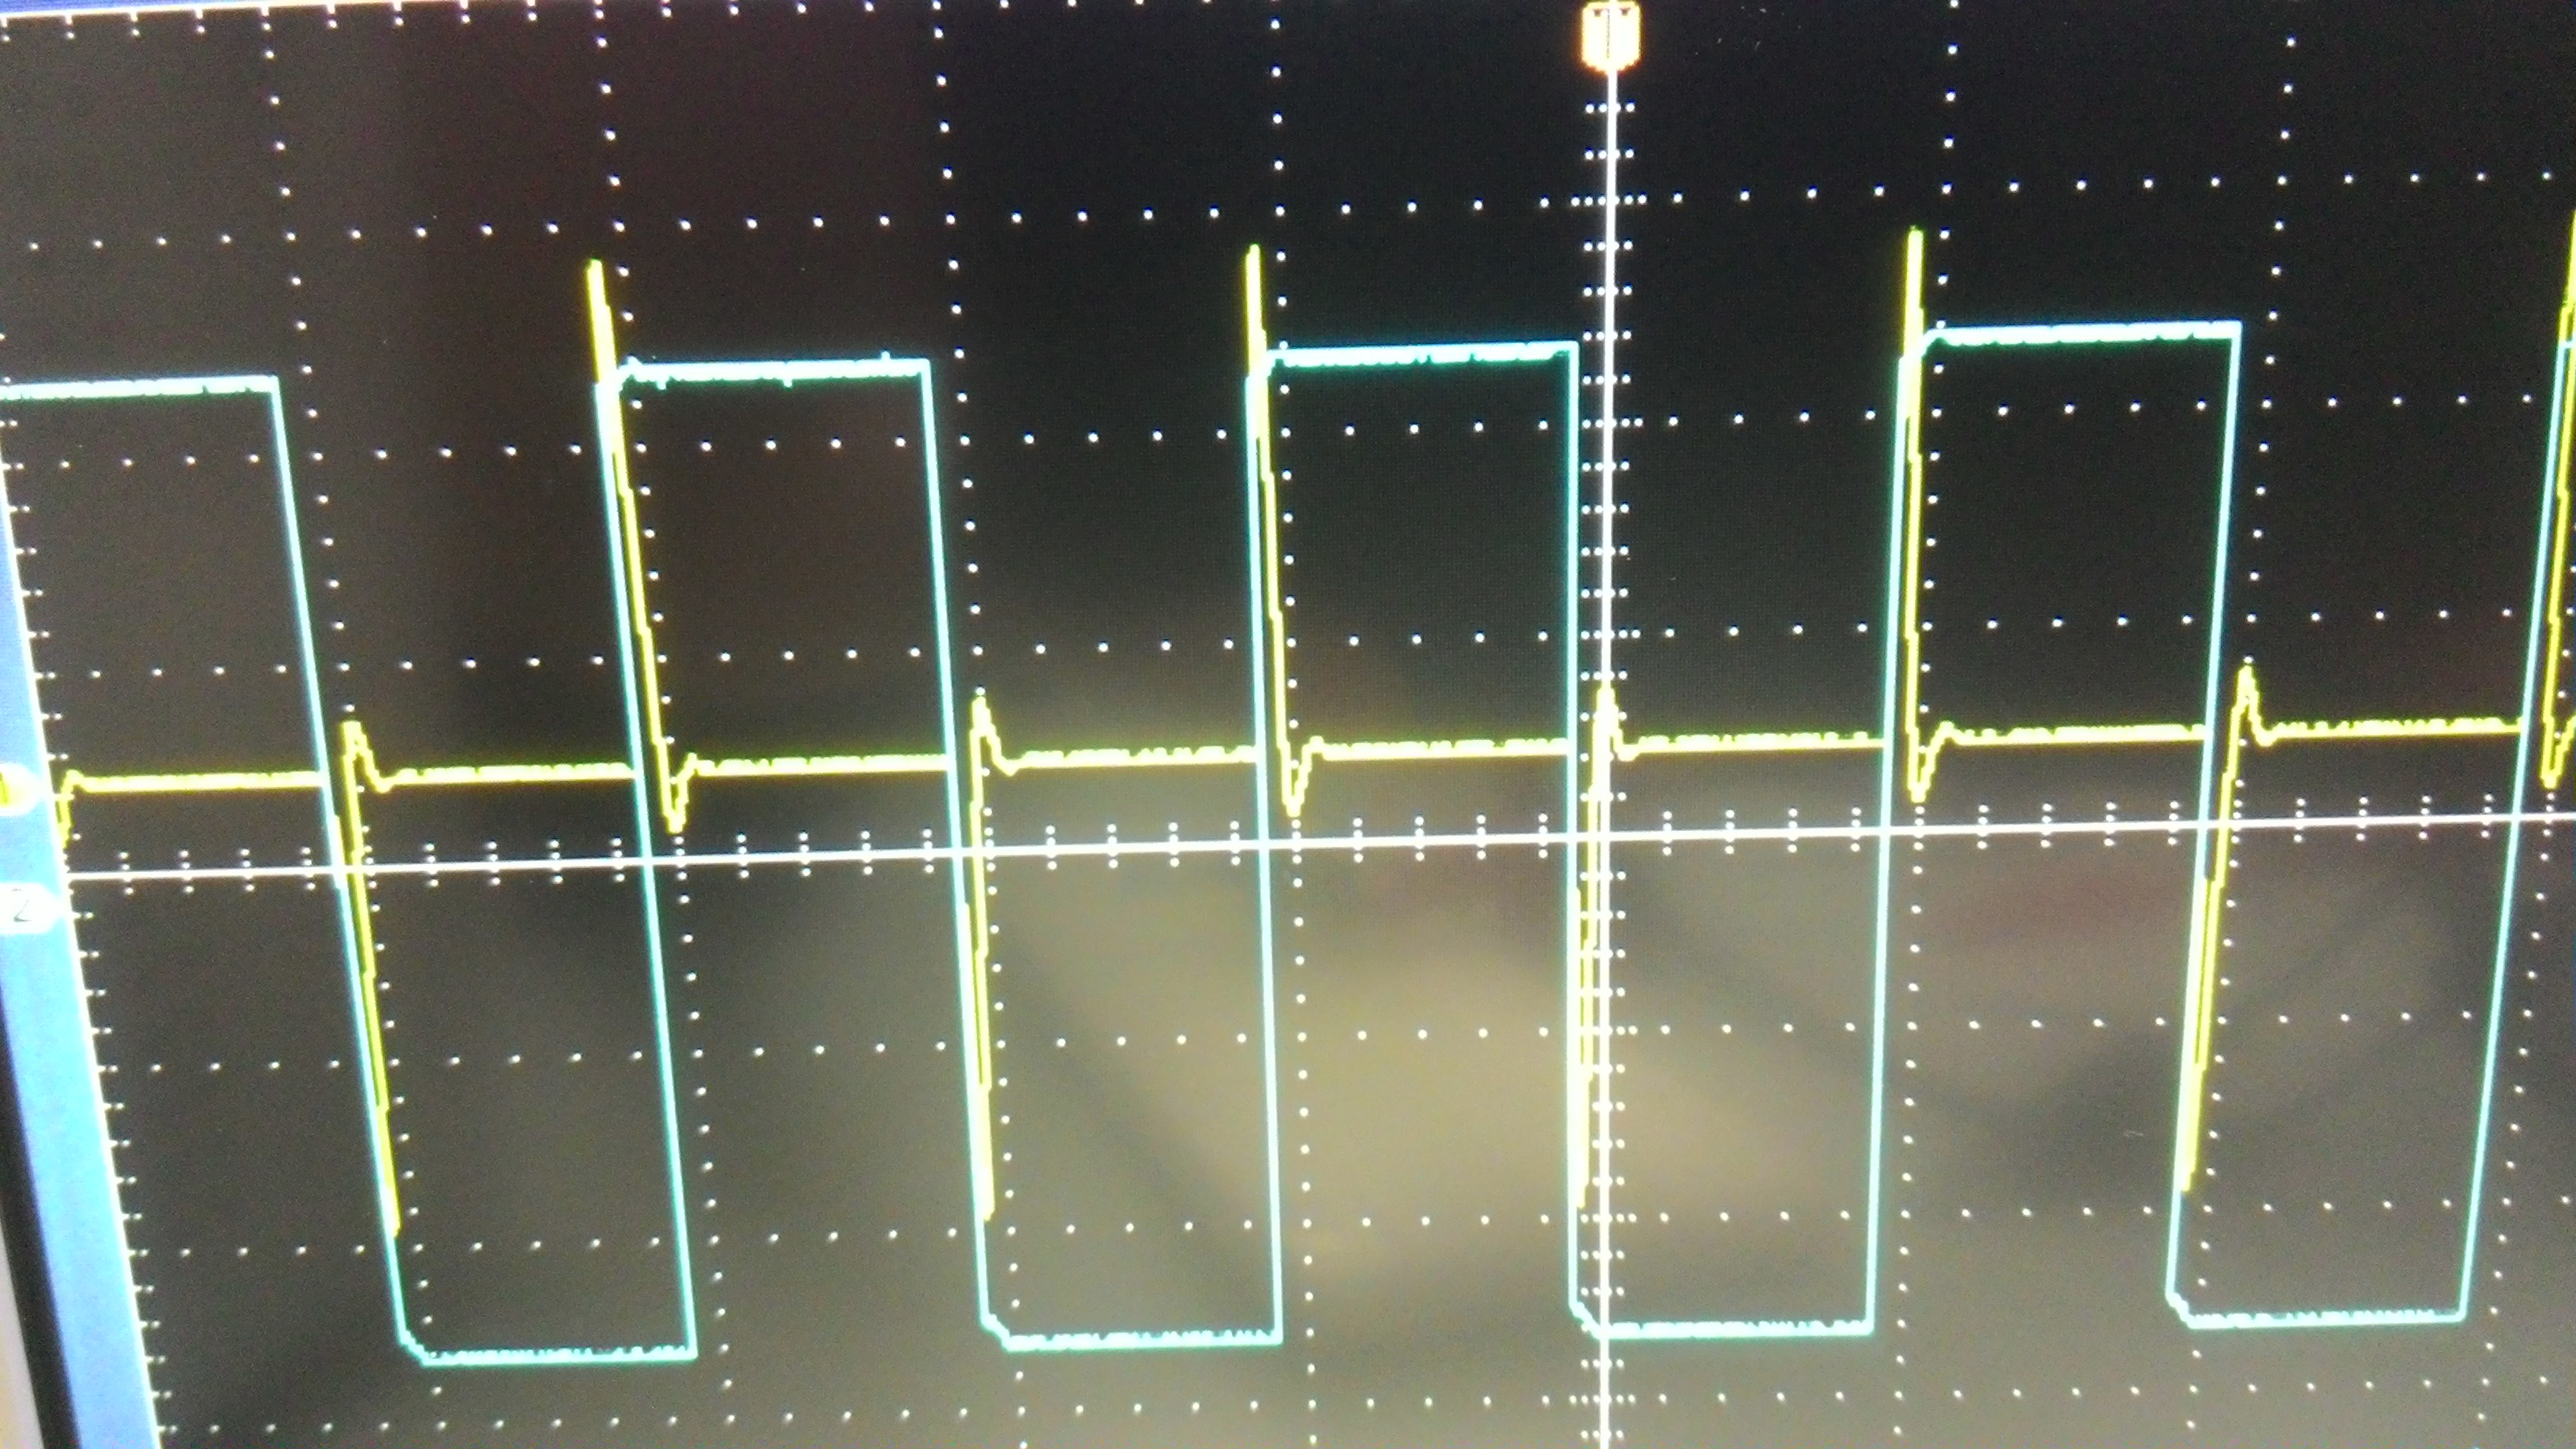
\includegraphics[width=1\textwidth]{data/pic/P_20141118_190528.jpg}
    \caption{$V_R$}
  \end{subfigure}
  \begin{subfigure}[b]{0.6\textwidth}
    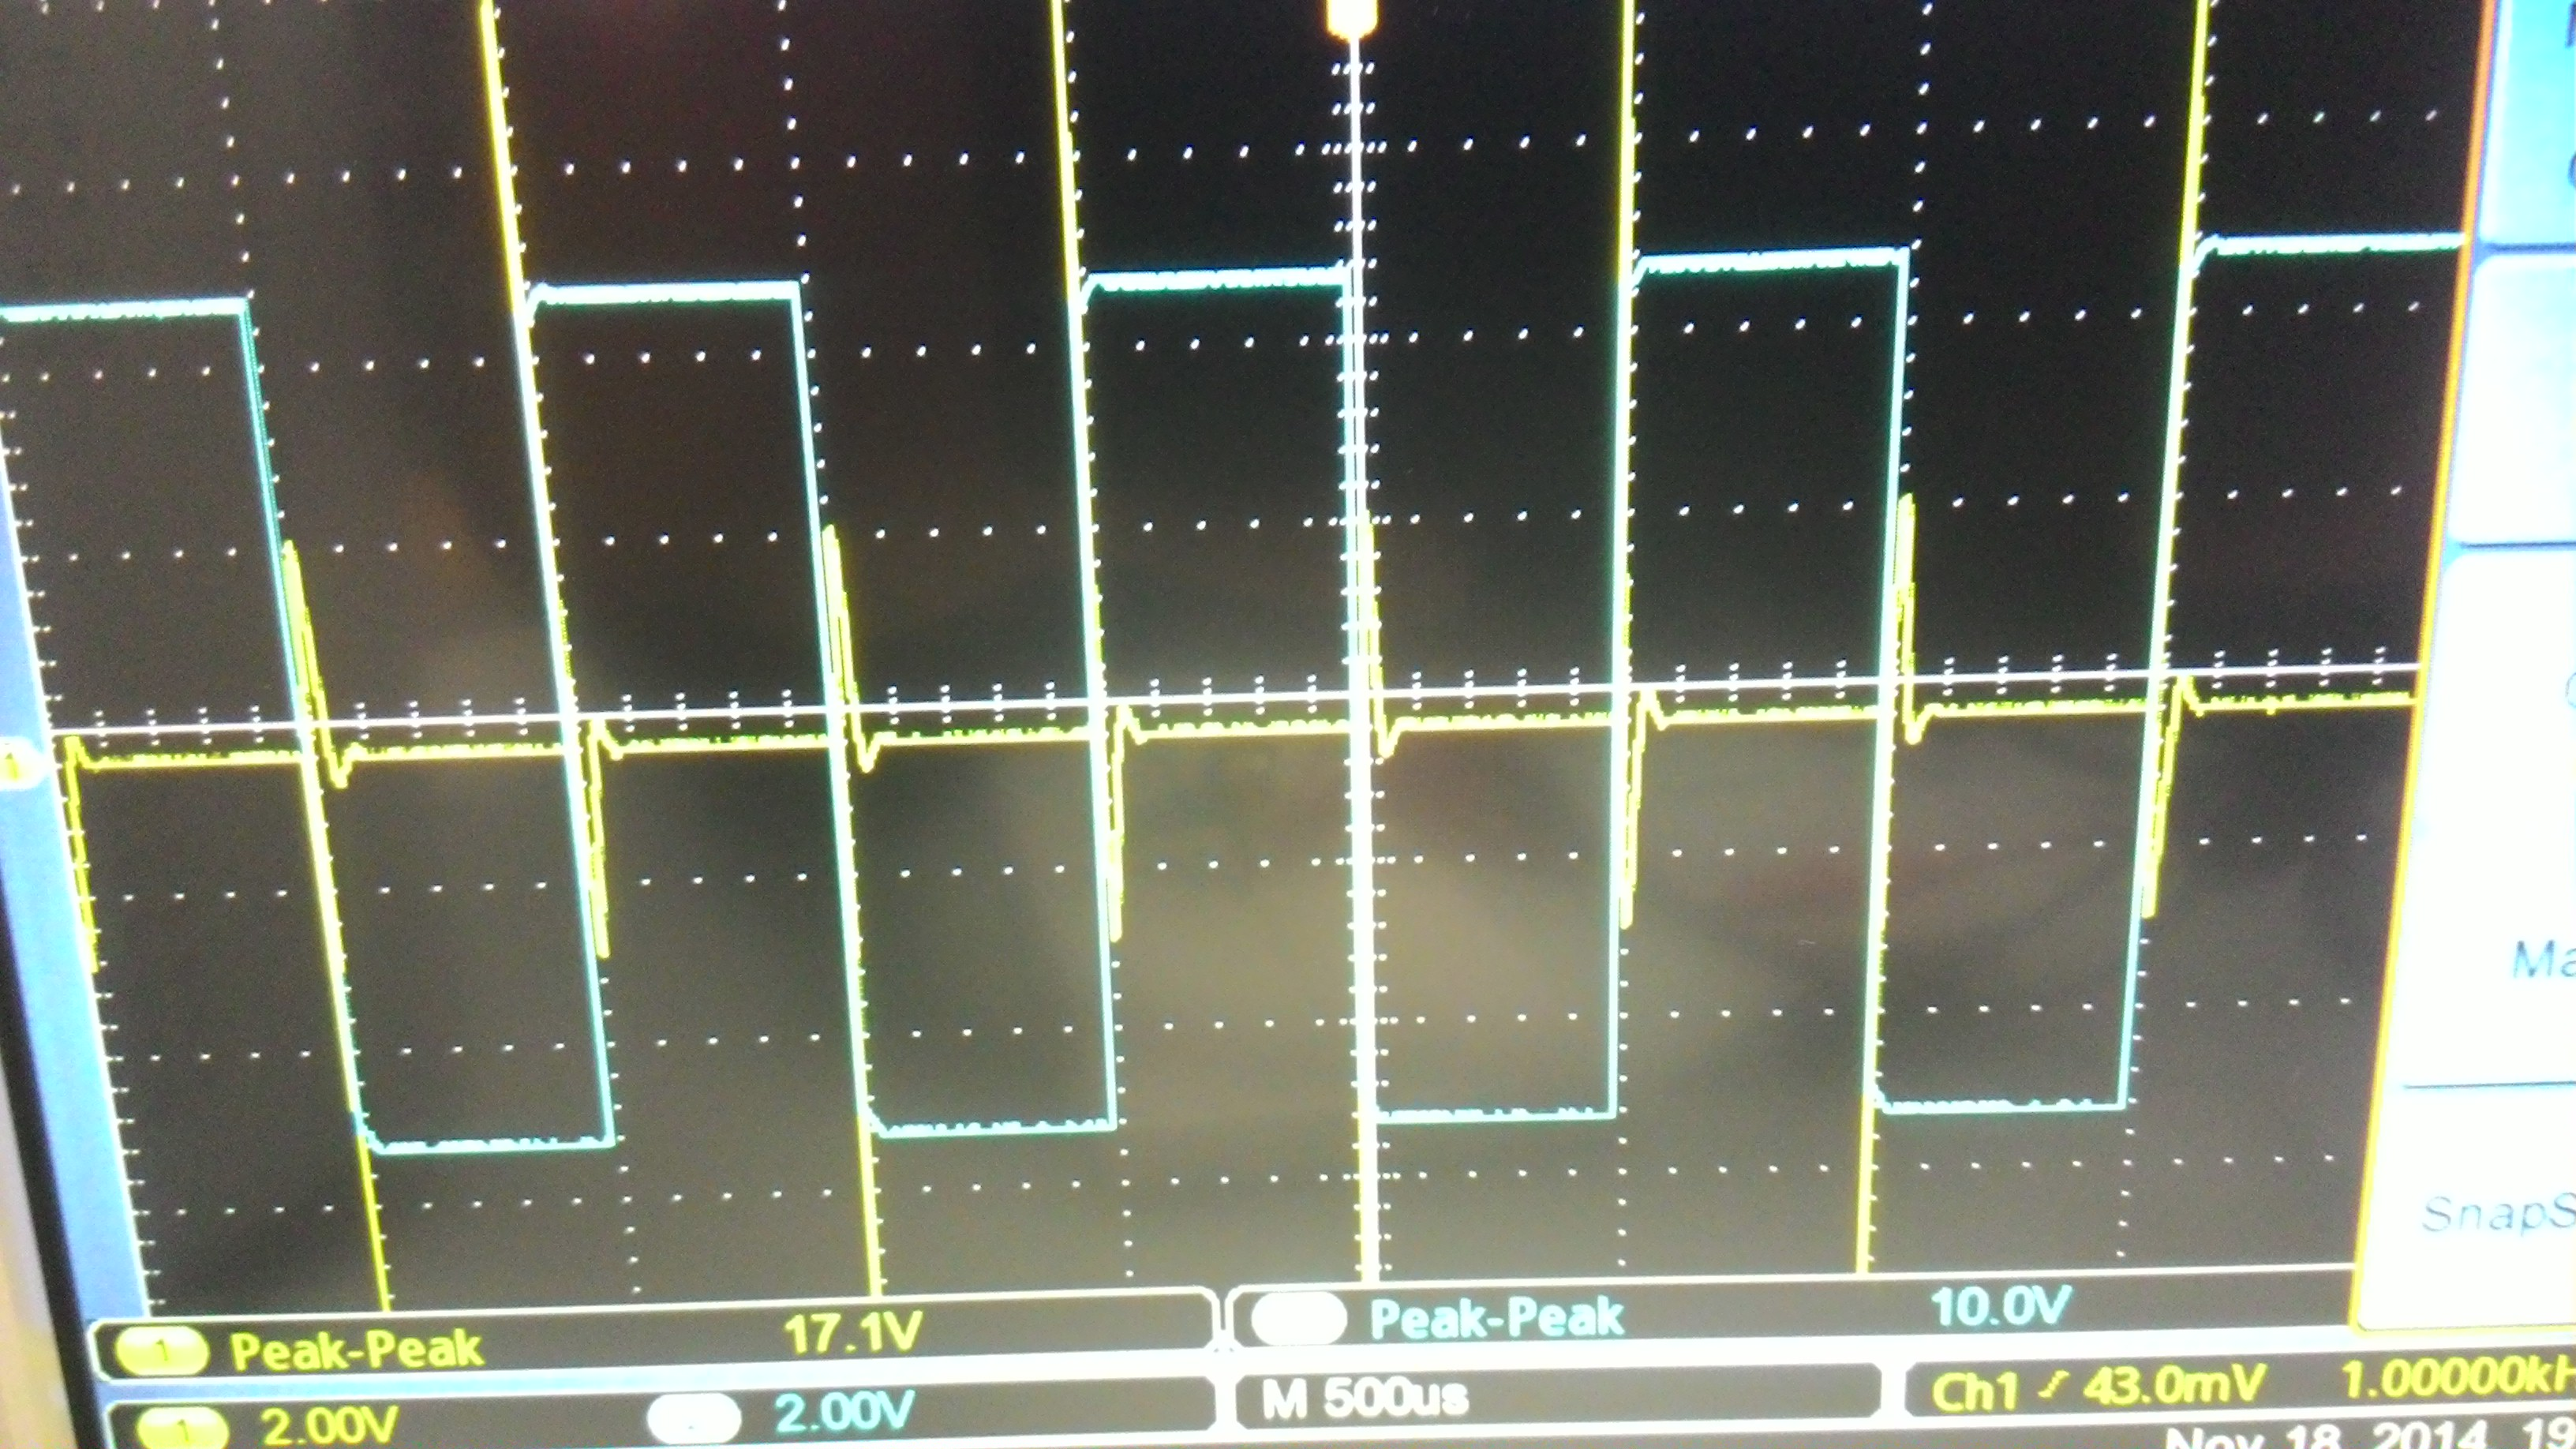
\includegraphics[width=1\textwidth]{data/pic/P_20141118_190803.jpg}
    \caption{$V_L$}
  \end{subfigure}
\end{figure}

\subsection{臨界阻尼}
\begin{figure}[H]
  \centering
  \begin{subfigure}[b]{0.6\textwidth}
    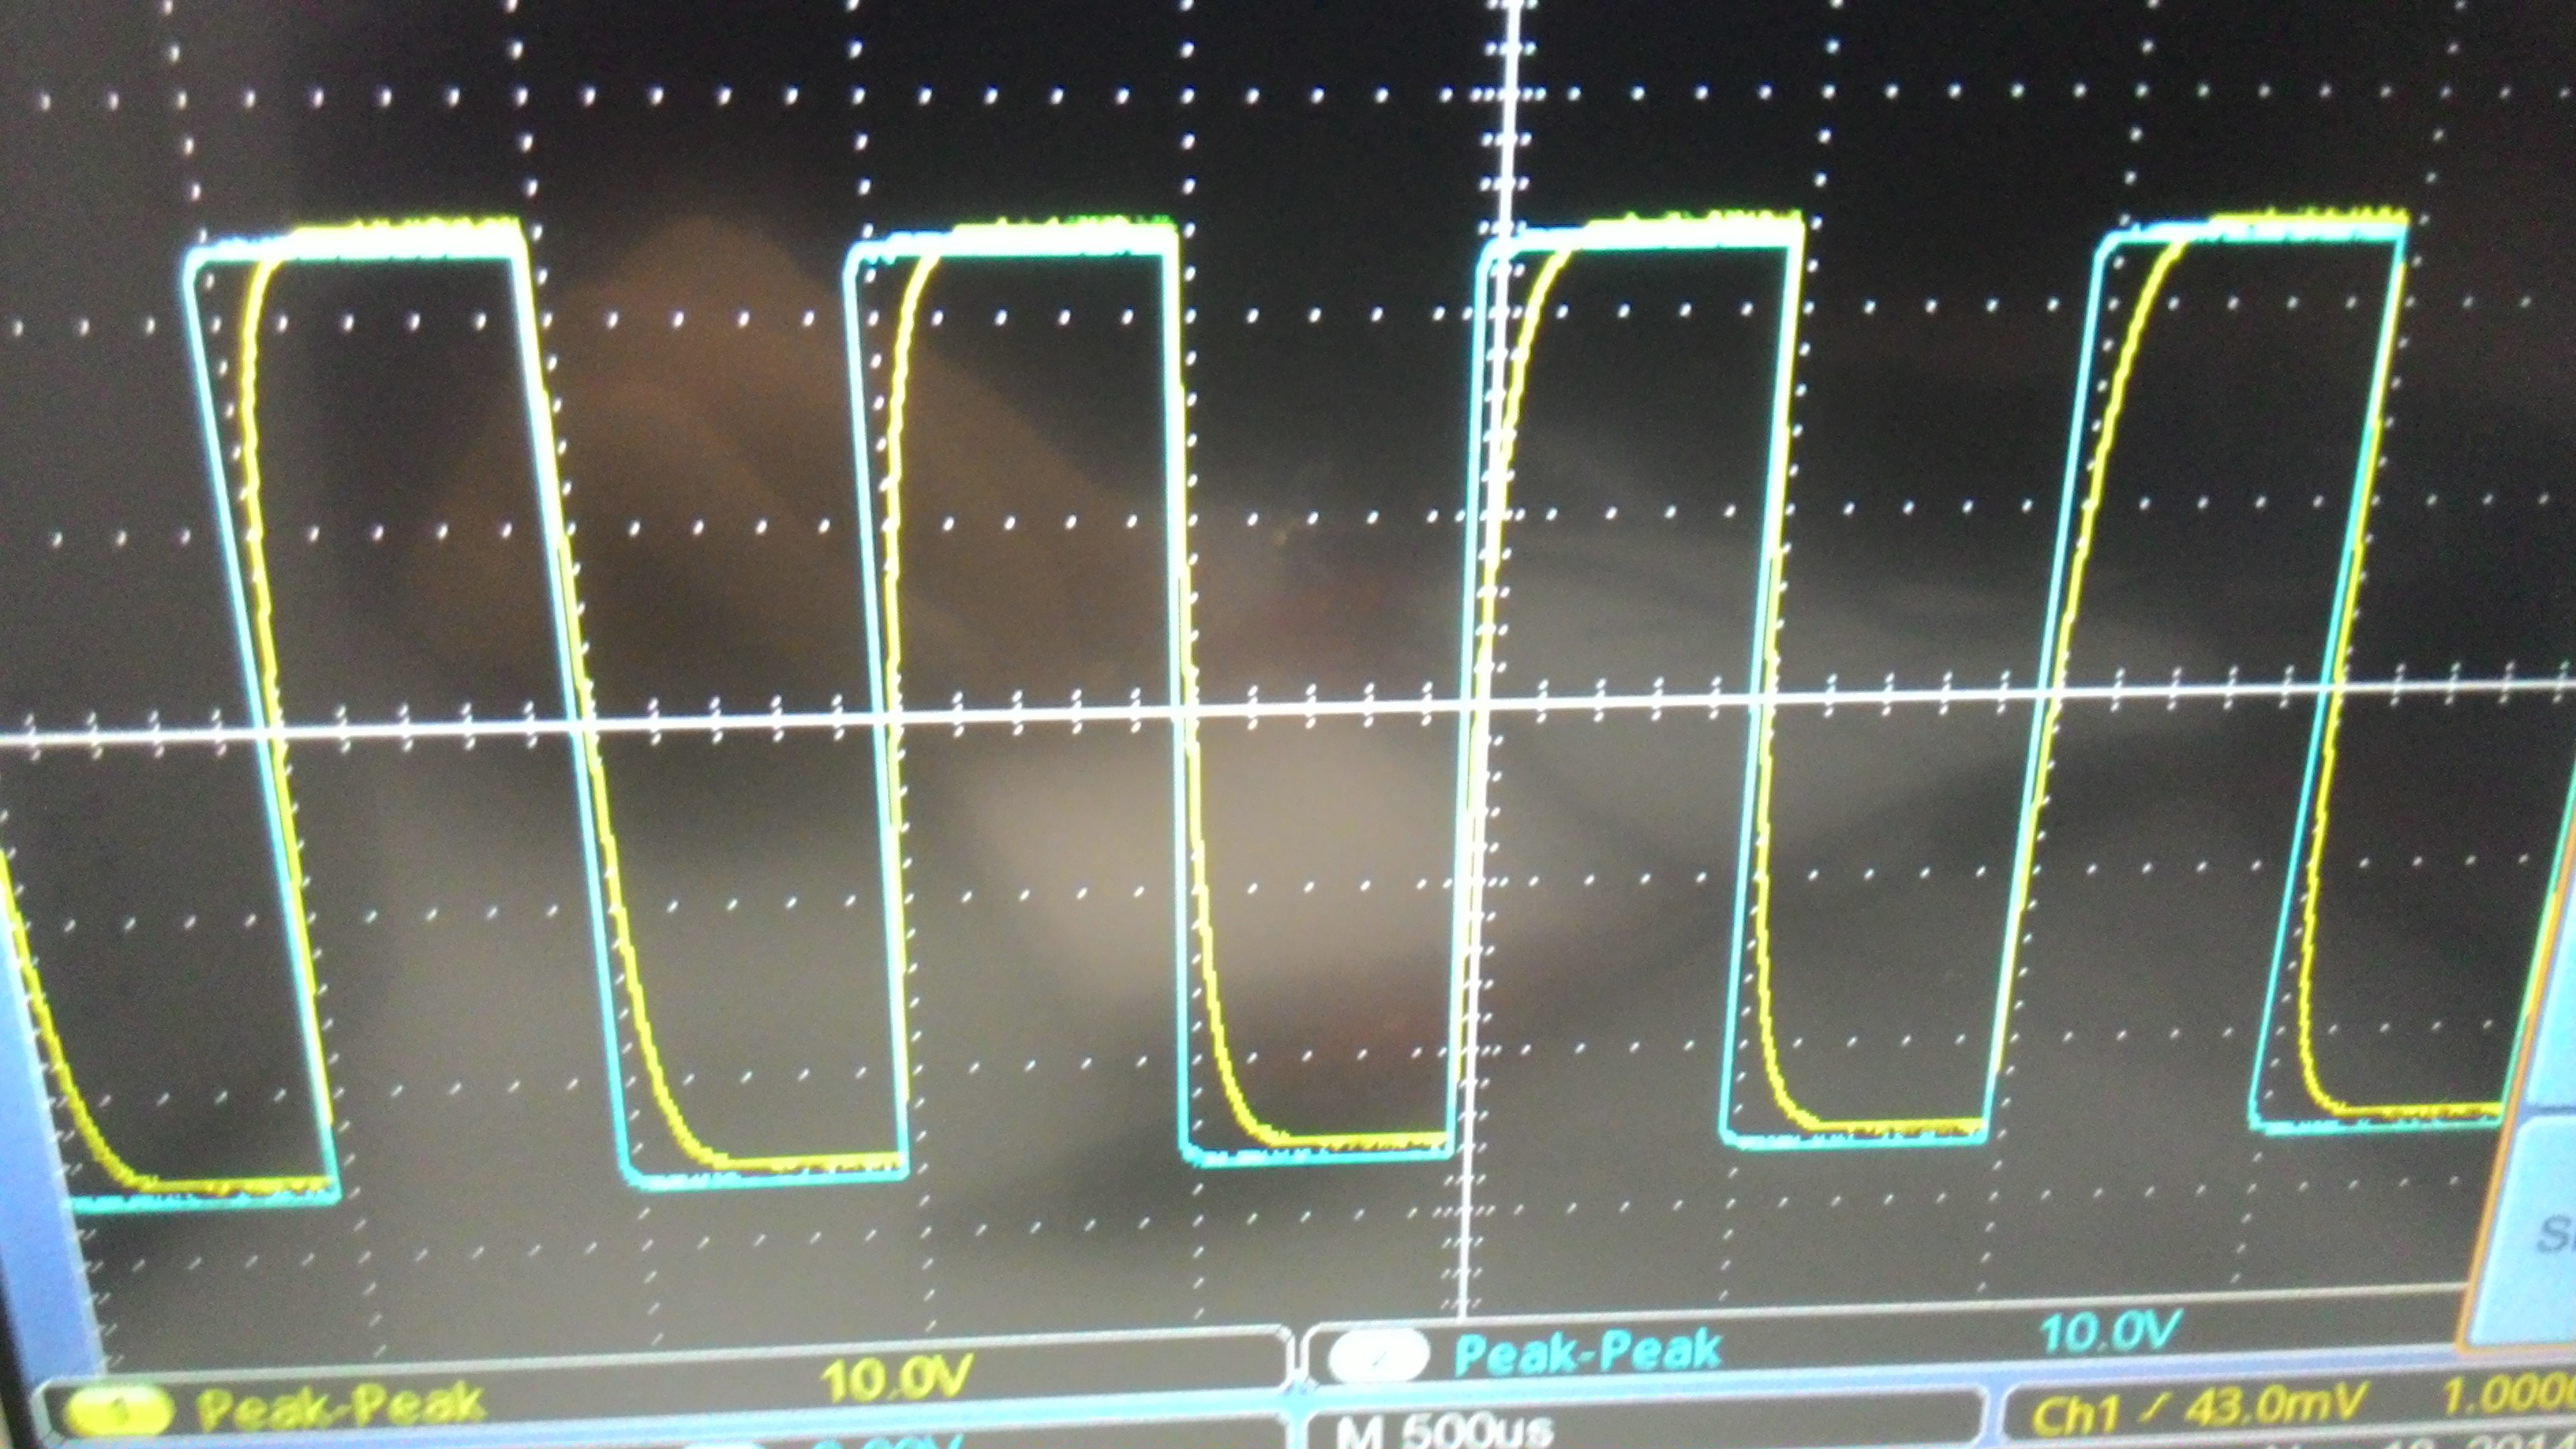
\includegraphics[width=1\textwidth]{data/pic/P_20141118_191631.jpg}
    \caption{$V_C$}
  \end{subfigure}
  \begin{subfigure}[b]{0.6\textwidth}
    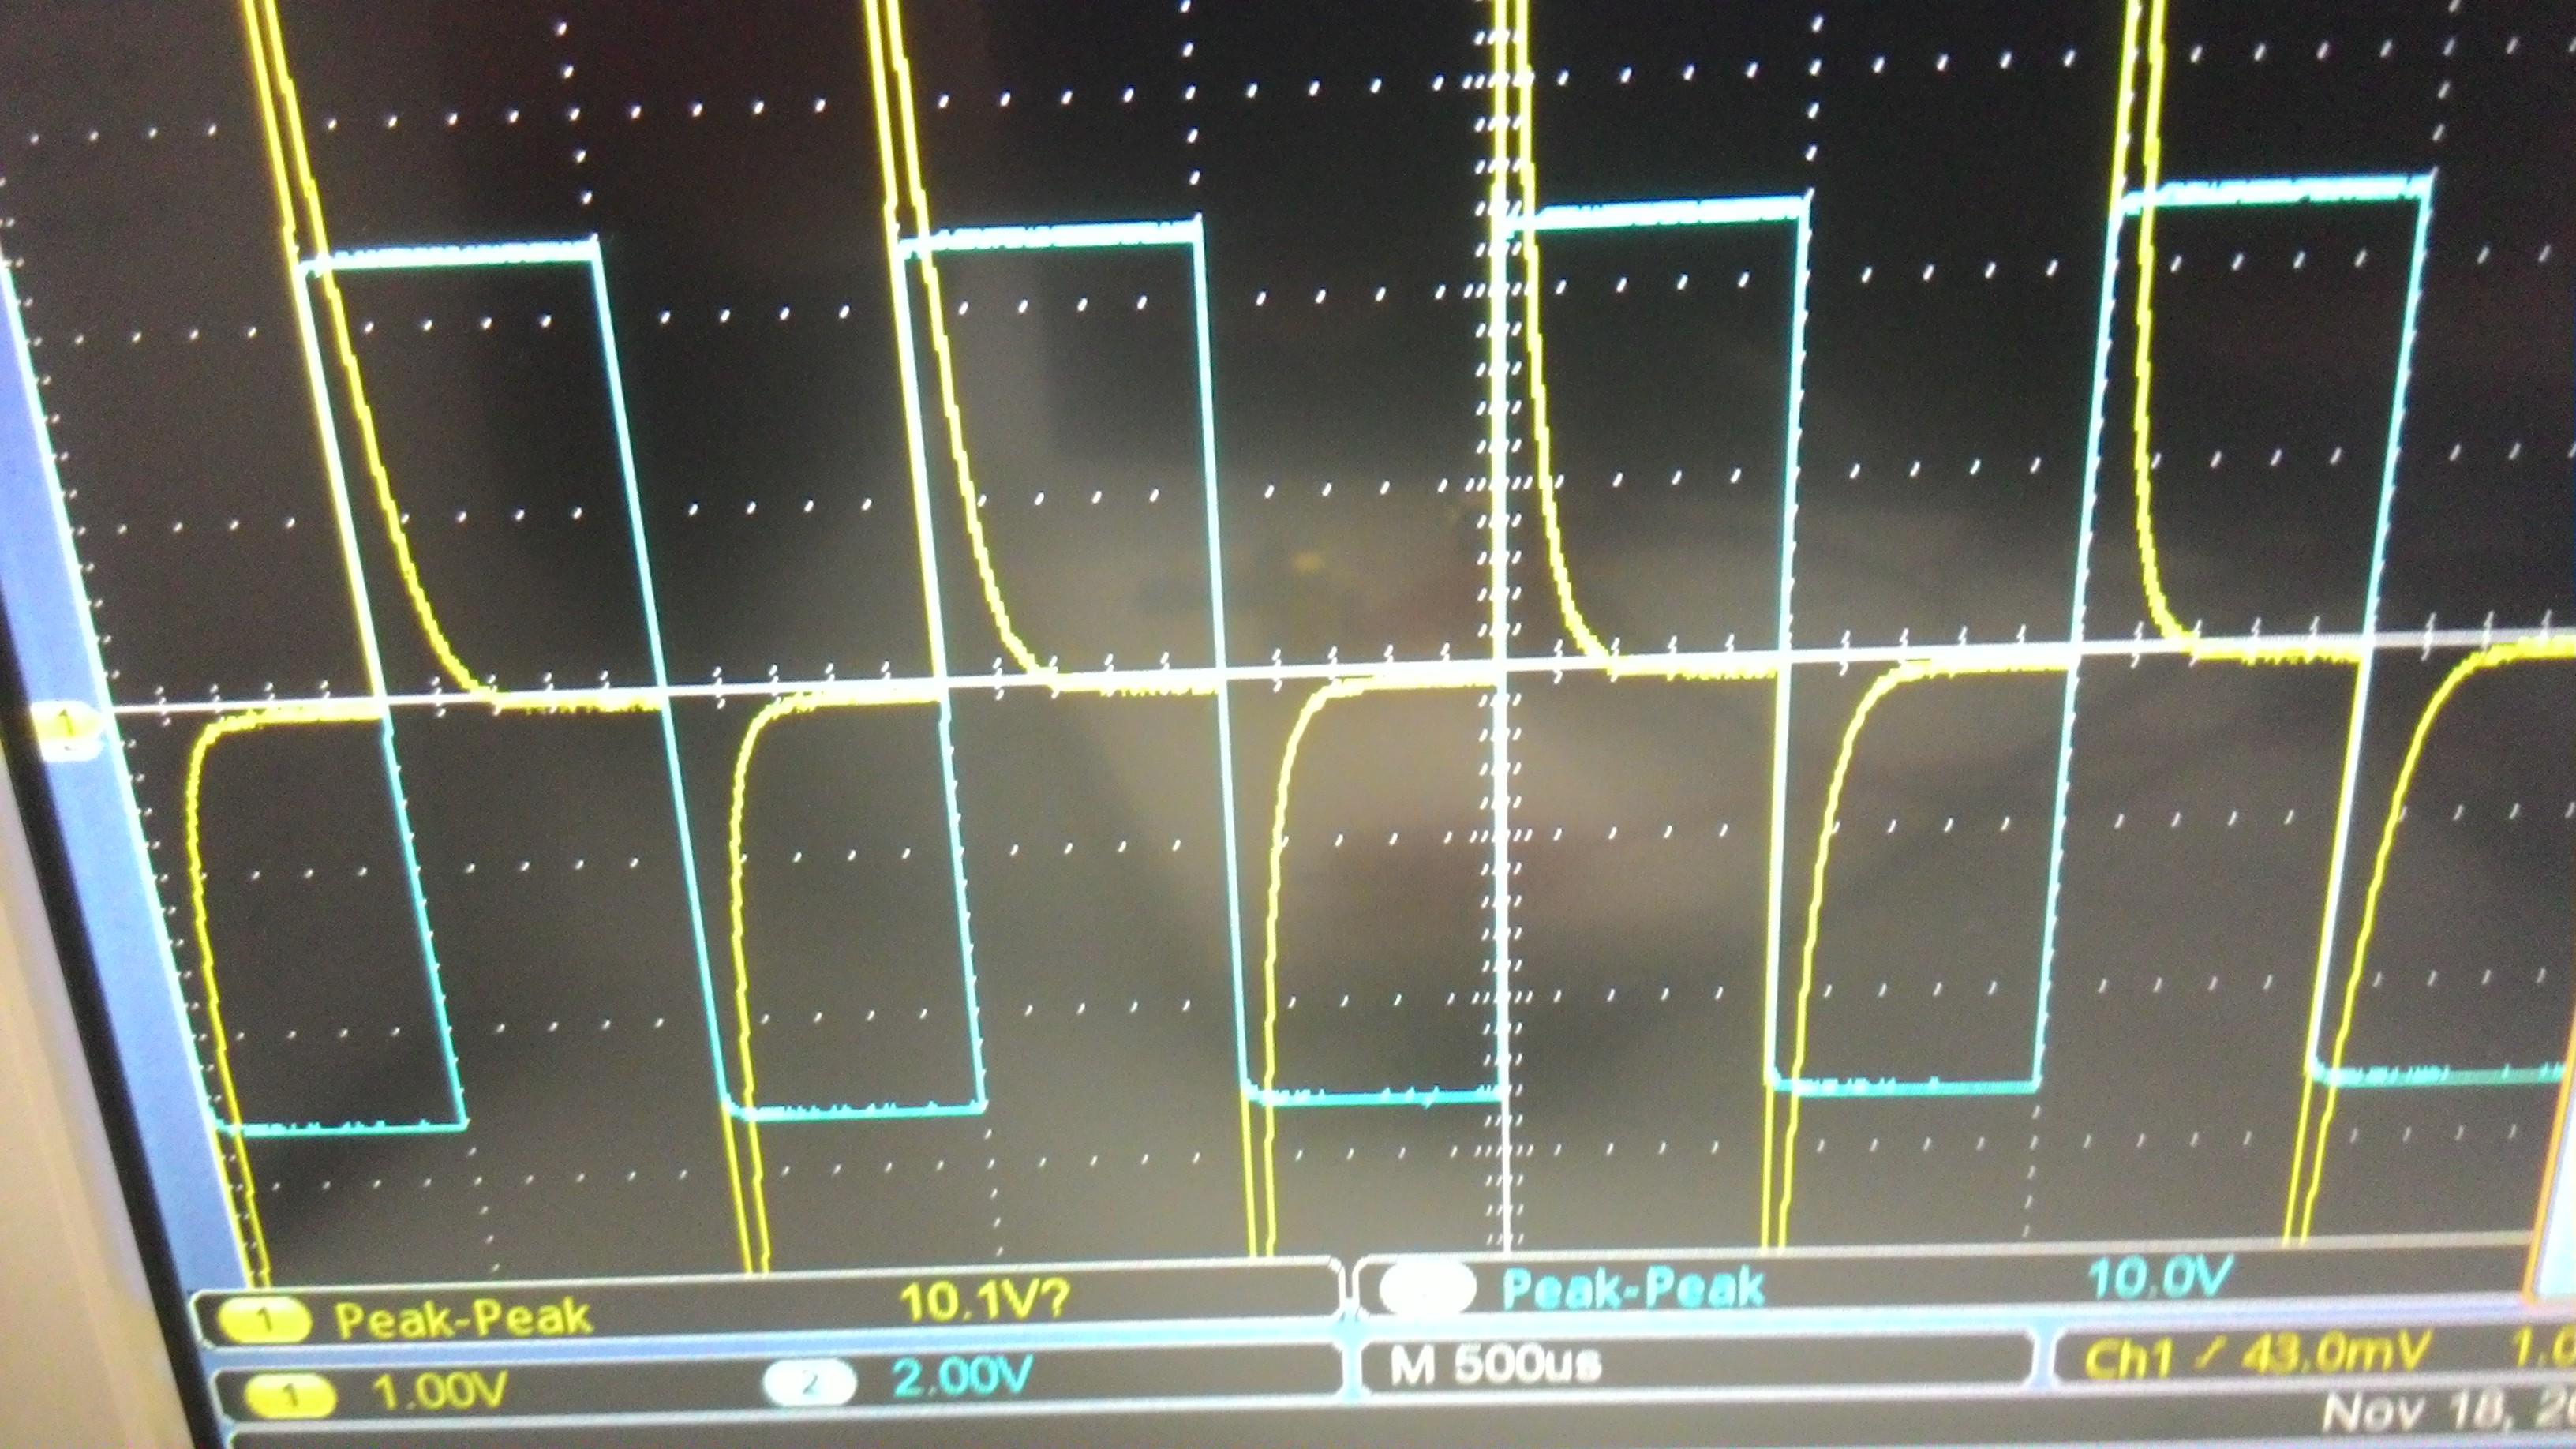
\includegraphics[width=1\textwidth]{data/pic/P_20141118_191610.jpg}
    \caption{$V_R$}
  \end{subfigure}
  \begin{subfigure}[b]{0.6\textwidth}
    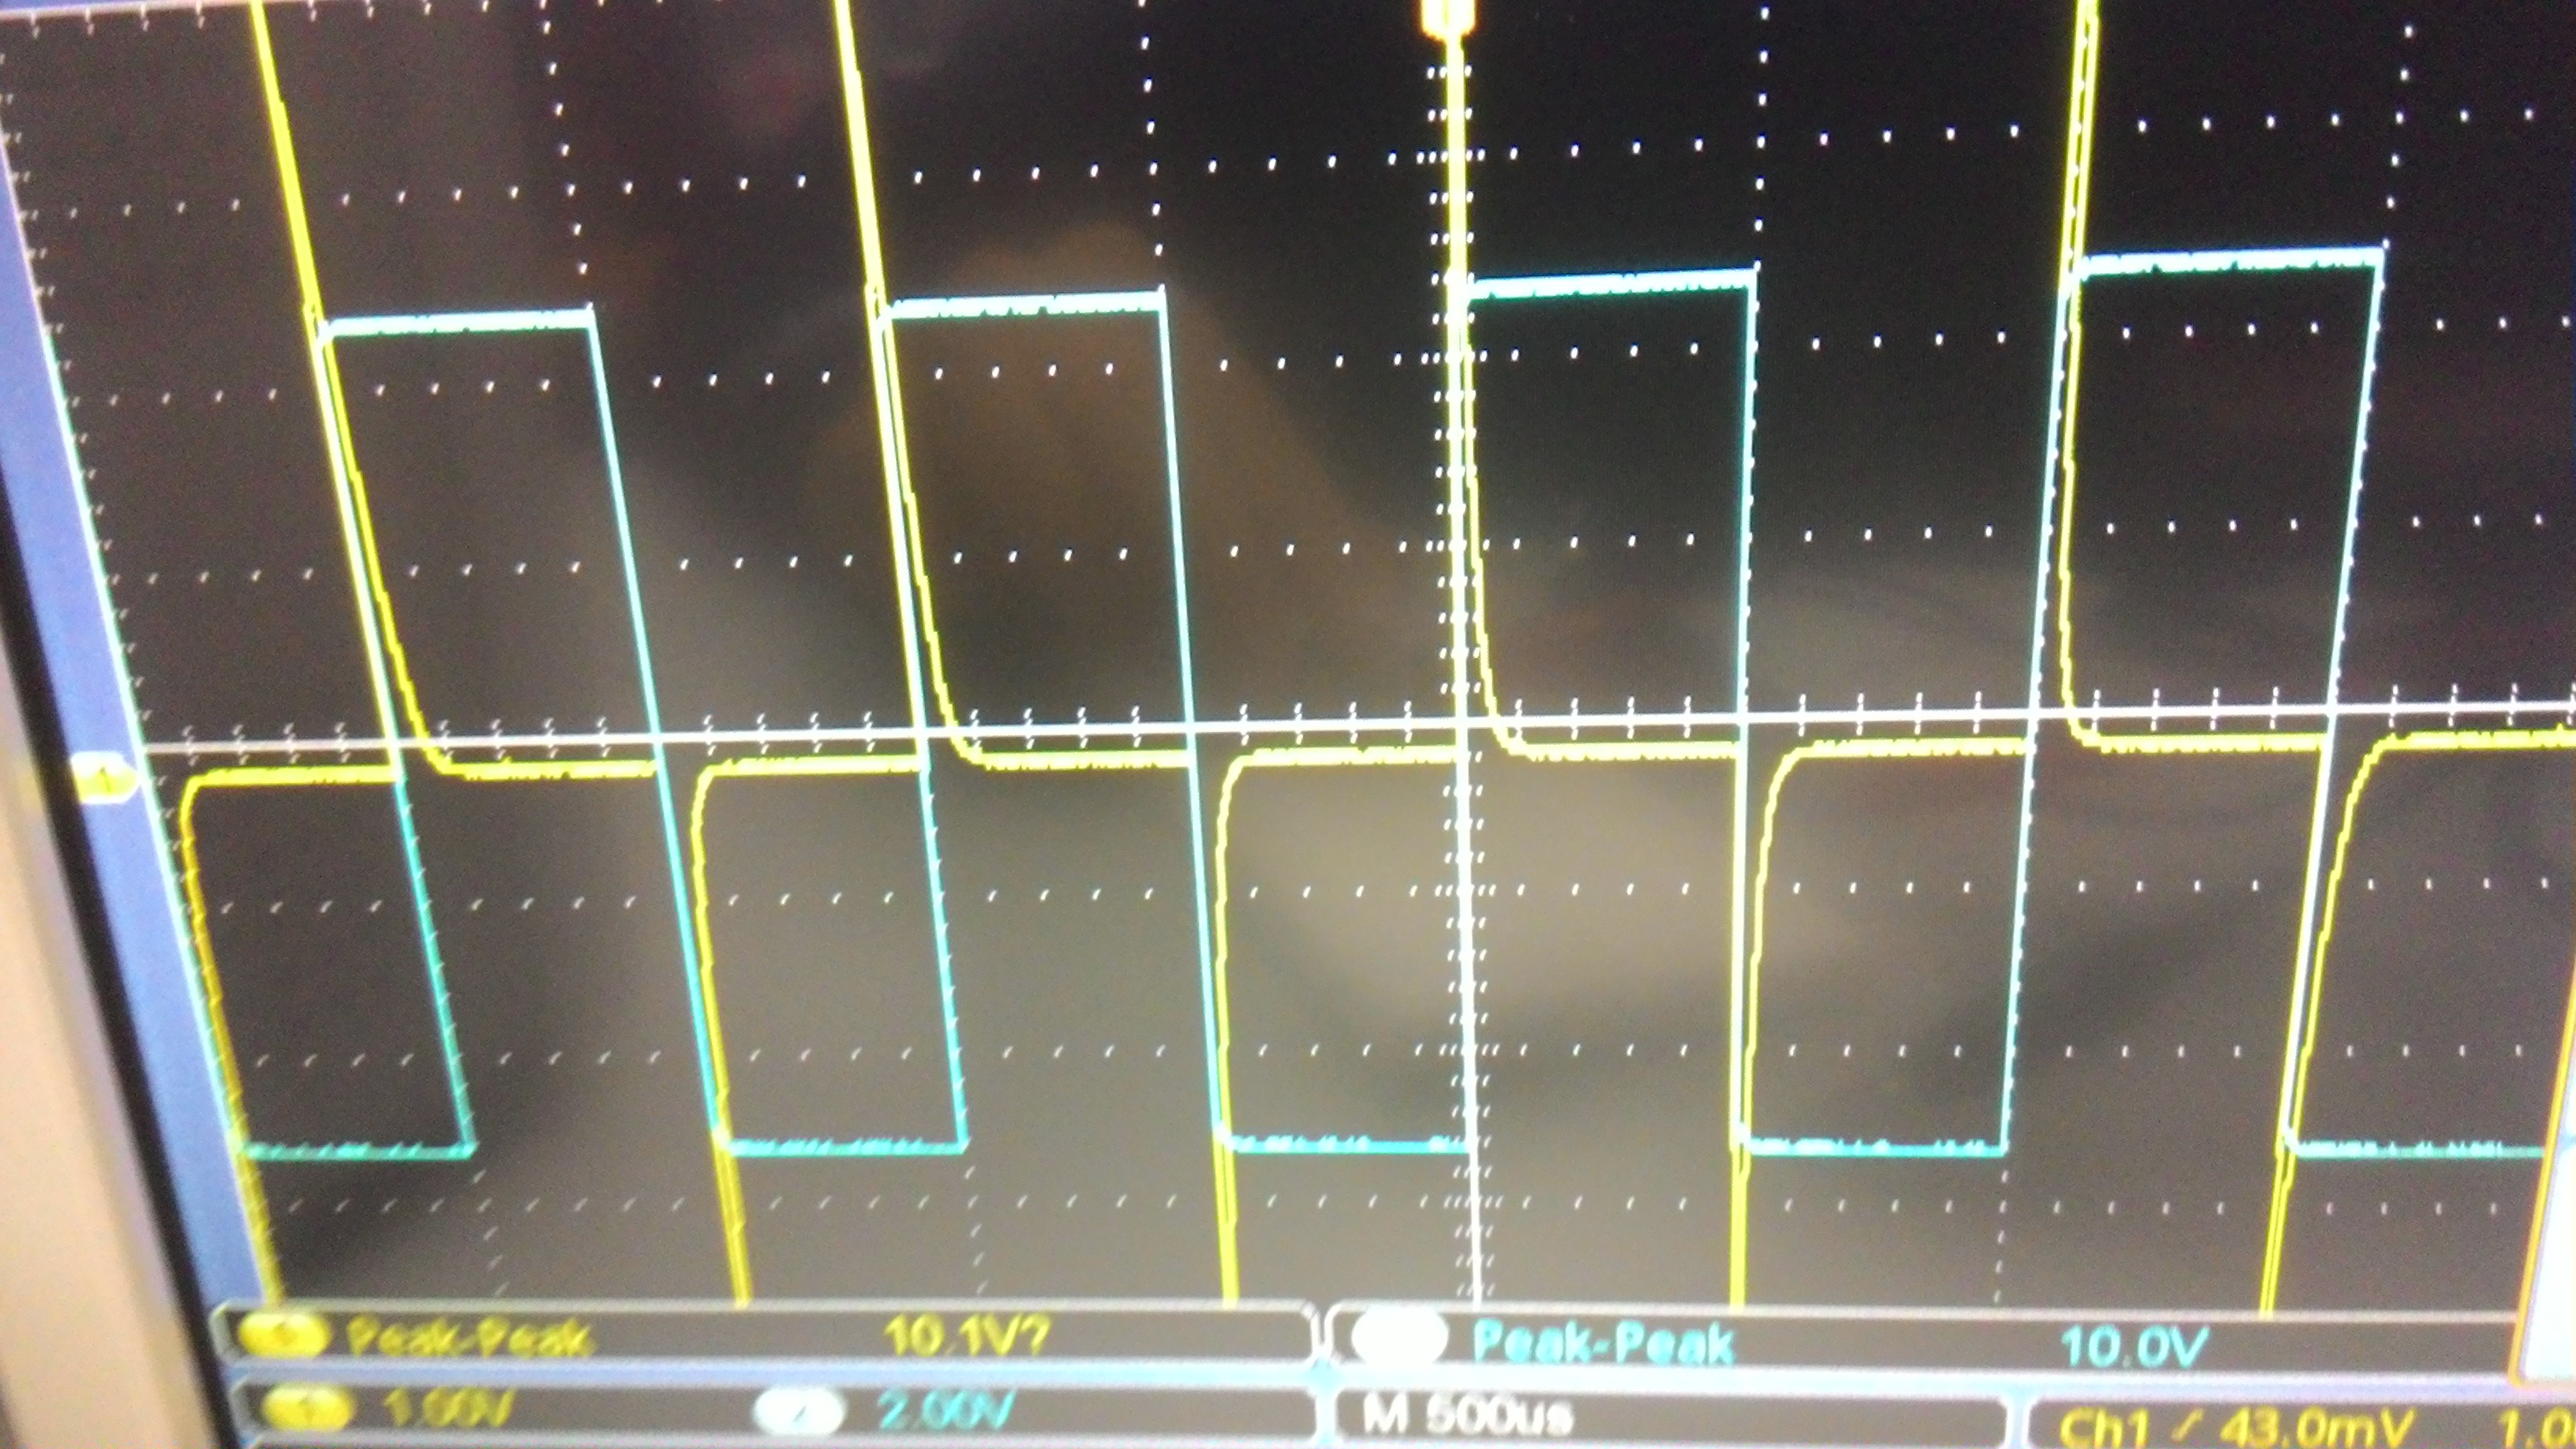
\includegraphics[width=1\textwidth]{data/pic/P_20141118_191333.jpg}
    \caption{$V_L$}
  \end{subfigure}
\end{figure}

\section{結報問題}

\begin{enumerate}[itemsep=20pt, topsep=10pt]
  \item {\large\bf 你所量出來的臨界阻尼R值較理論值為大或較理論值為小?為什麼會有這種情形發生?} \\[10pt]
    答: 所量測的臨界阻尼值較實驗值小,推測原因是電感內有不小的內電阻,假設臨界電阻為$R$,電感內的電阻為$R_L$,測我們測出的電阻會是$R - R_L < R$。另外臨界阻值的分界難以精確判斷,也是造成誤差的來源。
  \item {\large\bf 今若僅考慮元件本身(兩端各具一導線),不另考慮與環境其它元件之交互關係,請個別就電阻、電容與電感,繪出該元件與其寄生元件。} \\[10pt]

    \begin{figure}[H]
      \centering
\begin{tikzpicture}[american voltages, scale=.8, transform shape]
	\draw[color=black, thick]
  (0, 0) to [short] (0, 1) to [L, l=$R_A$] (0, 3) to [V] (0, 5) to [short] (0, 6)
  (0, 6) to [short] (1, 6) to [R, l=$R_L$] (3, 6) to [L, l=$L$] (5, 6) to [C, l=$C_L$] (7, 6) to[short] (8, 6)
  (8, 6) to [short] (8, 5) to [R, l=$R$] (8, 3) to [C, l=$C_R$] (8, 1) to [short] (8, 0)
  (8, 0) to [short] (6, 0) to [R, l=$C$] (2, 0) to [short] (0, 0)
  (0, 0) node[ground] {}
	;
  \draw (1, 5) rectangle (7, 7.5);
  \draw (4, 4.5) node[]{電感};
  \draw (7.2, 5) rectangle (9.5, 1);
  \draw (10, 3) node[]{電阻};
  \draw (3, -1) rectangle (5, 1);
  \draw (4, 1.5) node[]{電容};
\end{tikzpicture}
    \end{figure}
  
  如上圖,因電阻內材質不同,會有少量電容產生,而電感本身就有不小的電阻(也因此有微小的電容)。最後,整個電路也會有一個微小的電感$L_A$。

\end{enumerate}

\section{心得}
一開始做實驗時,打開抽屜一看,不知道為啥電路線只剩下寥寥可數的幾條。後來只好去沒有人做的抽屜偷拿幾條,才發現原來座位也有分權貴等級的,有些位置的麵包板是全新的,有些看起來能用就偷笑了。看來座位也要挑個風水好一點的。
\end{document}

